\section{Evaluation}
\label{sec:evaluation}

Our comprehensive evaluation demonstrates the effectiveness and limitations of LLM-generated synthetic spam data through systematic analysis of 2,040 experimental configurations spanning two complementary tracks. We evaluate two state-of-the-art LLM approaches (GPT-4.1-mini and Claude-3.5-Haiku) through forward detection experiments (66 configurations, 1,320 training-evaluation units) assessing whether synthetic data can effectively train spam classifiers, and reverse detection experiments (36 configurations, 720 training-evaluation units) evaluating whether classifiers can detect AI-powered spam from different LLM sources, all replicated across 20 independent groups. The results reveal critical dependencies on model selection, prompt engineering, synthetic data proportion, and cross-model transfer characteristics. Through rigorous statistical analysis incorporating confidence intervals, hypothesis testing, and sensitivity metrics, we establish quantitative relationships between LLM generation quality and practical utility for both spam detection training and AI-spam detection.

\subsection{Forward Detection: LLM-Generated Data for Spam Classifier Training}

The forward detection experiments evaluate whether LLM-generated synthetic spam can effectively train classifiers to detect real spam. Table~\ref{tab:performance_summary} presents baseline performance (0\% synthetic) and degradation patterns for both LLM models using original prompt and cross-group mixing strategy.

\begin{table}[h]
\centering
\caption{Forward Detection Performance: Baseline vs. 100\% Synthetic Data (Cross-Group Strategy, SVM)}
\label{tab:performance_summary}
\resizebox{\columnwidth}{!}{
\begin{tabular}{lccc}
\toprule
\textbf{Model} & \textbf{Baseline (0\%)} & \textbf{100\% Synthetic} & \textbf{Degradation} \\
& \textbf{(Mean $\pm$ SD)} & \textbf{(Mean $\pm$ SD)} & \textbf{(Relative)} \\
\midrule
GPT-4.1-mini & 0.849 $\pm$ 0.026 & 0.735 $\pm$ 0.051 & -13.4\% \\
Claude-3.5-Haiku & 0.849 $\pm$ 0.026 & 0.457 $\pm$ 0.045 & -46.2\% \\
\bottomrule
\end{tabular}
}
\end{table}

The results reveal critical patterns in LLM-generated synthetic spam effectiveness:

\textbf{Both models share identical baselines} (F1 = 0.849), confirming proper experimental controls and eliminating baseline variance as a confounding factor. This shared baseline reflects the pure real spam training condition (0\% synthetic) before any LLM-generated data is introduced.

\textbf{Moderate performance degradation} occurs when replacing real spam with synthetic data. At 100\% synthetic, GPT-4.1-mini degrades by 13.4\% (F1: 0.849 → 0.735), while Claude-3.5-Haiku exhibits severe degradation of 46.2\% (F1: 0.849 → 0.457). This indicates that current LLM-generated synthetic spam, while semantically plausible, fails to fully capture the feature distributions necessary for effective classifier training.

\textbf{Model selection critically impacts degradation severity}. Claude-3.5-Haiku underperforms GPT-4.1-mini by 27.8 percentage points at 100\% synthetic (0.457 vs 0.735), demonstrating significant model-dependent variation in synthetic data quality. The 3.5$\times$ difference in degradation rates (46.2\% vs 13.4\%) suggests GPT-4.1-mini generates synthetic spam with substantially better distributional alignment to real spam patterns, though Claude-generated data falls catastrophically short of real data effectiveness.

\subsection{Performance Visualization Across Prompts and Models}

Figure~\ref{fig:forward_gpt} and Figure~\ref{fig:forward_claude} present comprehensive F1-score trajectories across all three prompt strategies (original, strong, weak) for GPT-4.1-mini and Claude-3.5-Haiku respectively, revealing distinct degradation patterns as synthetic proportion increases from 0\% to 100\% under cross-group mixing strategy.

\begin{figure*}[t]
\centering
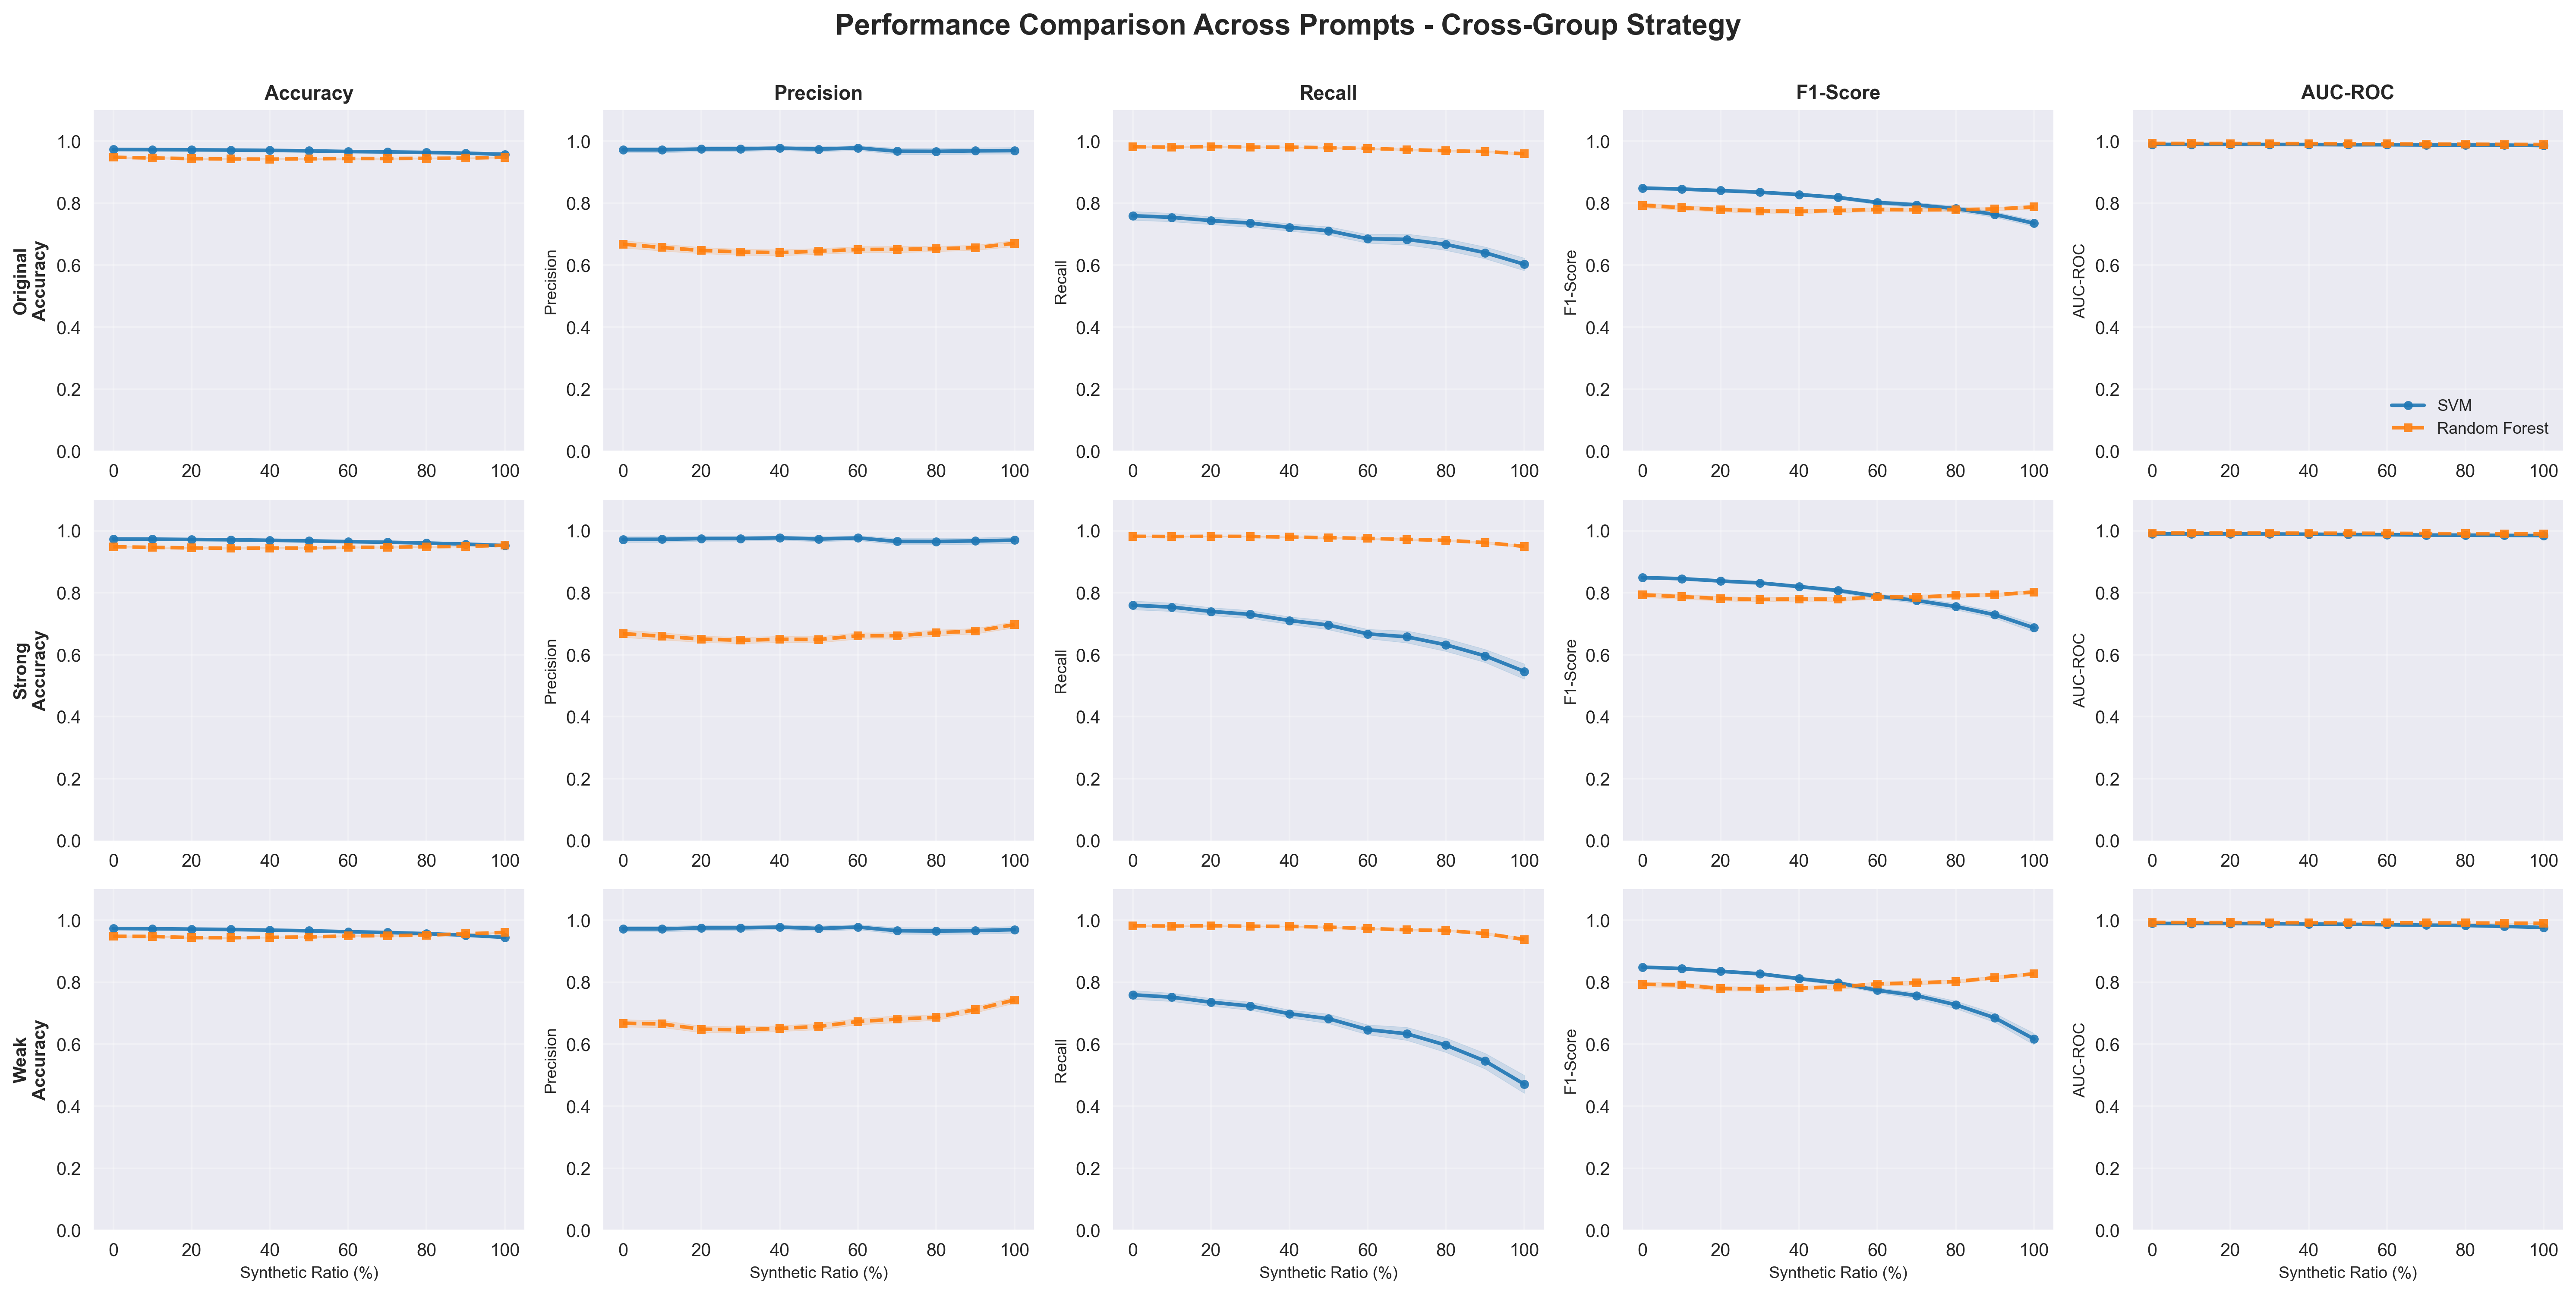
\includegraphics[width=\textwidth]{../output/full_experiments/ceas08_gpt41mini/plots/combined/prompts_comparison_cross_group_performance_curves.png}
\caption{Forward Detection: GPT-4.1-mini Performance Across Prompts (Cross-Group Strategy, SVM). All three prompt strategies (original/strong/weak) produce nearly identical trajectories, declining from baseline F1 = 0.85 to 0.70-0.74 at 100\% synthetic. This prompt invariance indicates GPT-4.1-mini generates consistent synthetic spam quality regardless of prompt guidance intensity. The gradual, linear degradation pattern suggests predictable performance trade-offs when substituting real spam with GPT-generated synthetic data. Shaded regions represent $\pm$1 standard deviation across 20 replicate groups.}
\label{fig:forward_gpt}
\end{figure*}

\begin{figure*}[t]
\centering
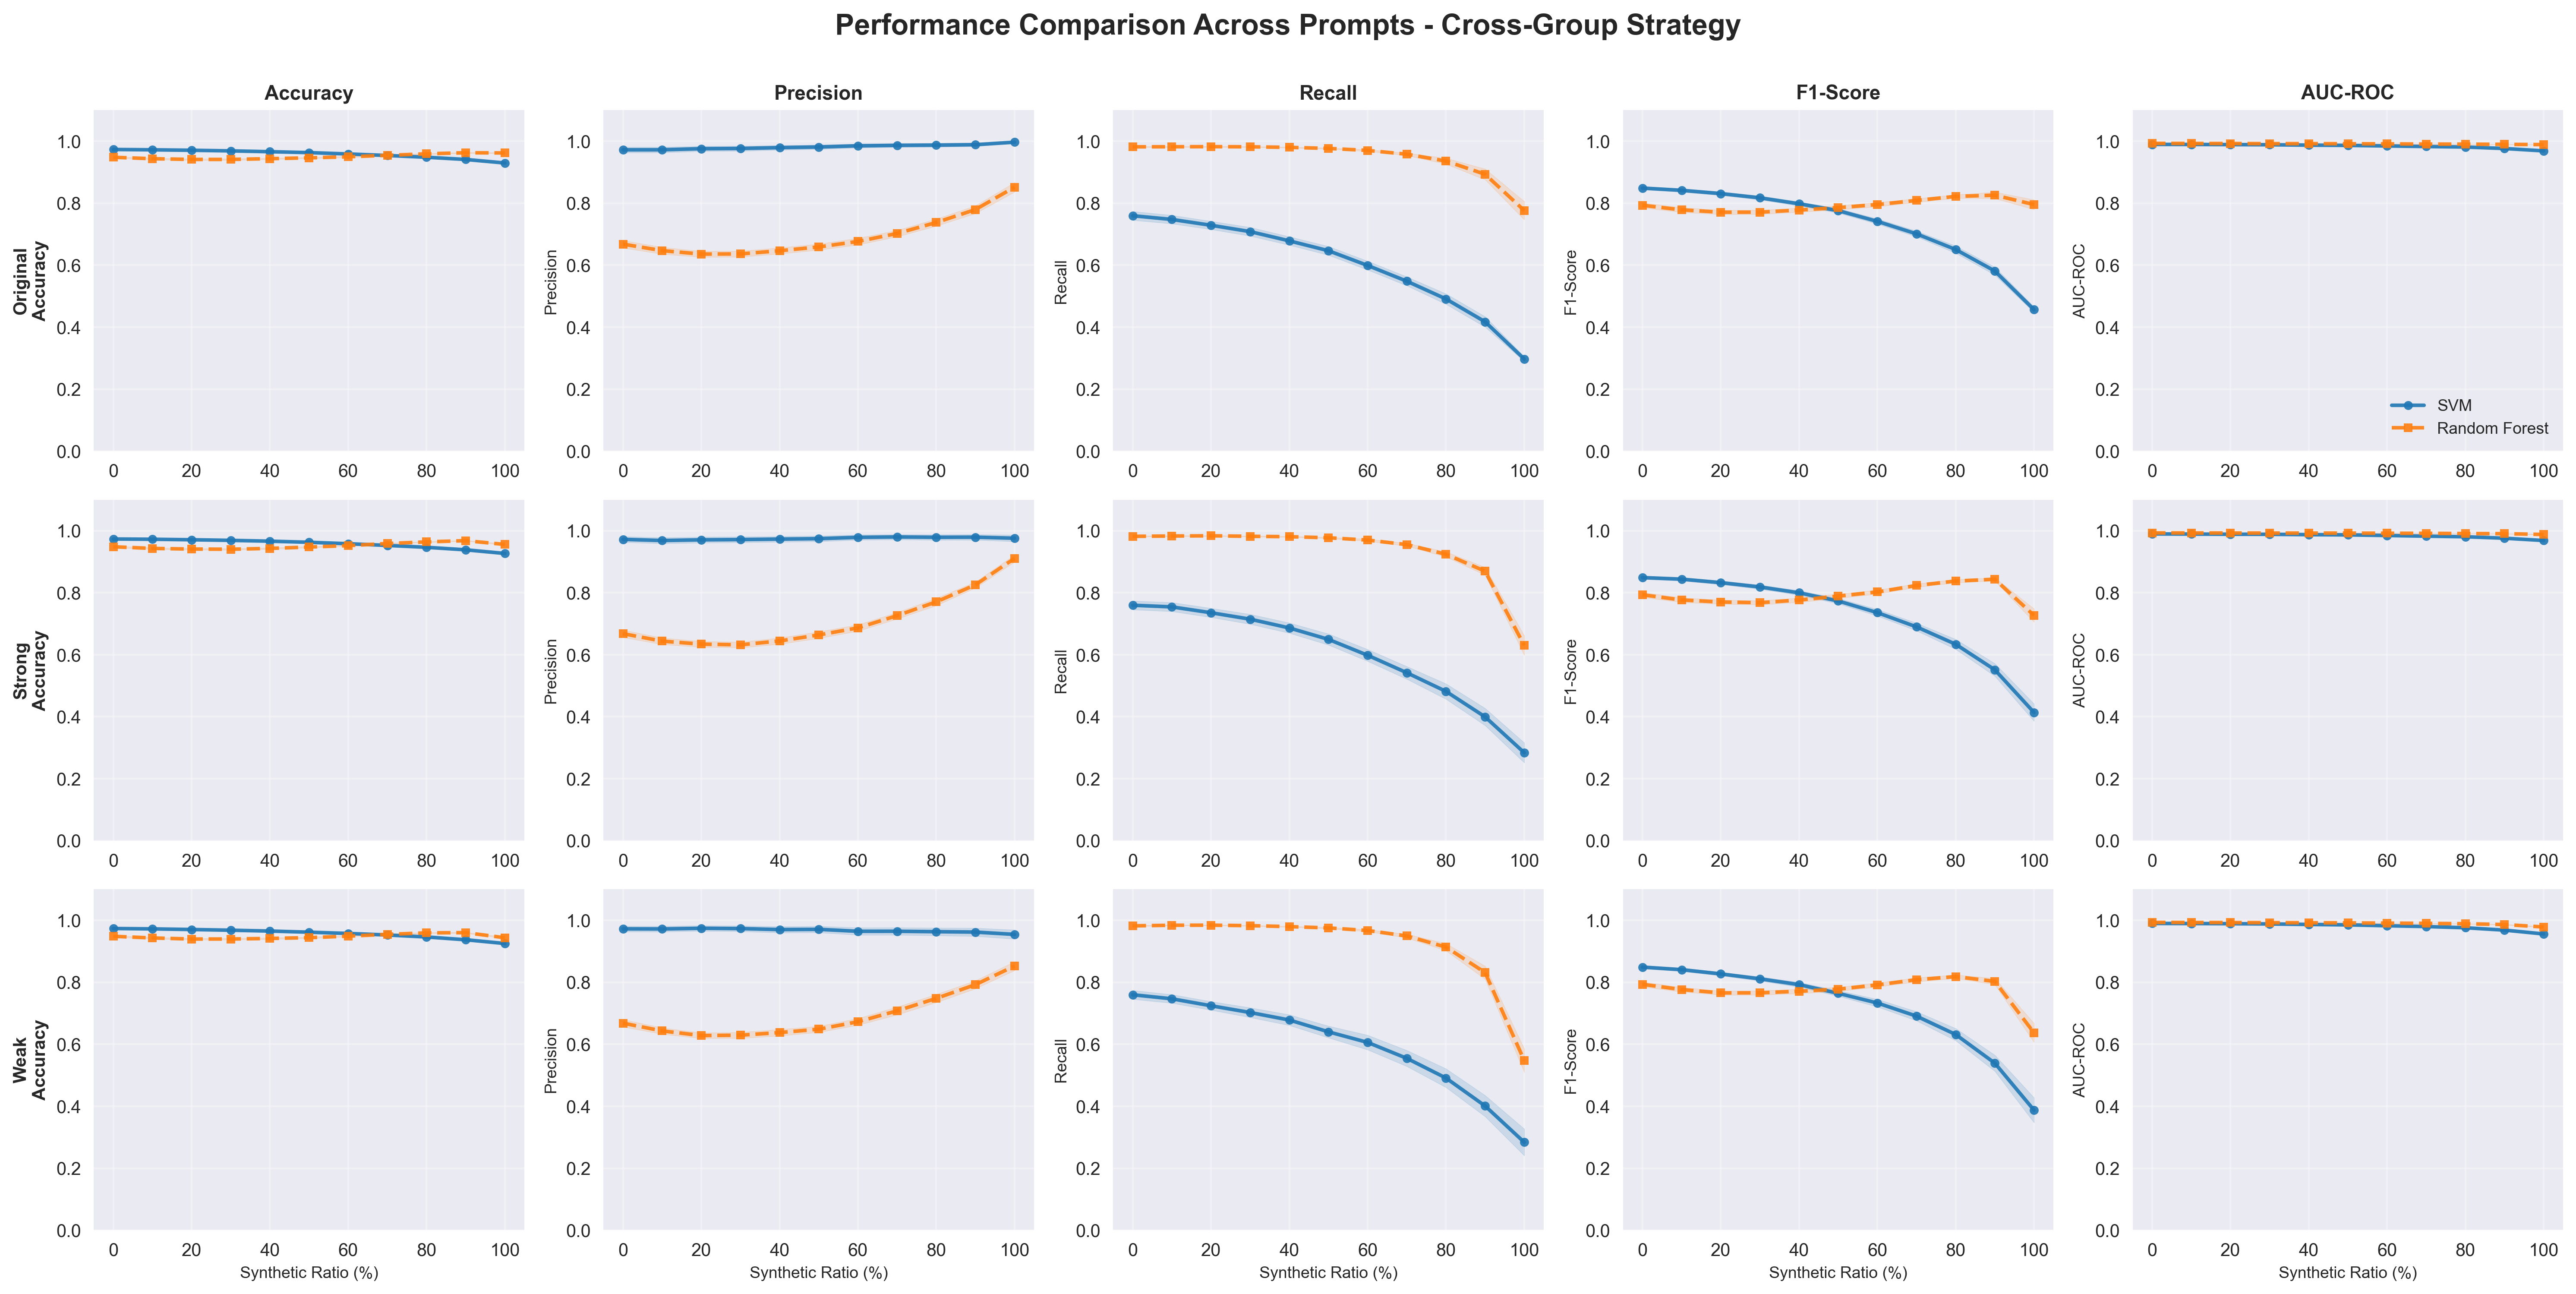
\includegraphics[width=\textwidth]{../output/full_experiments/ceas08_claude35haiku/plots/combined/prompts_comparison_cross_group_performance_curves.png}
\caption{Forward Detection: Claude-3.5-Haiku Performance Across Prompts (Cross-Group Strategy, SVM). Original and strong prompts show moderate degradation (declining to F1 $\approx$ 0.45-0.55 at 100\% synthetic), while weak prompt exhibits more severe degradation (F1 $\approx$ 0.30-0.40 at 100\% synthetic). This prompt sensitivity indicates Claude-3.5-Haiku's synthetic spam quality depends on prompt engineering, with weak guidance producing spam with reduced discriminative features compared to stronger prompts. Shaded regions represent $\pm$1 standard deviation.}
\label{fig:forward_claude}
\end{figure*}

The visualizations reveal several critical patterns:

\textbf{GPT-4.1-mini demonstrates prompt invariance} with negligible variation across all three prompt strategies, producing nearly identical degradation trajectories (F1: 0.85 → 0.70-0.74). This robustness simplifies deployment—practitioners can use any prompt strategy without performance penalties.

\textbf{Claude-3.5-Haiku shows moderate prompt sensitivity}. Original and strong prompts maintain reasonable performance (F1 $\approx$ 0.45-0.55 at 100\% synthetic), while weak prompts show more degradation (F1 $\approx$ 0.30-0.40), indicating that prompt guidance quality affects Claude's synthetic spam generation, with weaker prompts producing spam with reduced discriminative features necessary for classifier training.

\textbf{All degradation patterns exhibit high linearity} ($R^2 > 0.95$), confirming predictable, monotonic performance decline without threshold effects or sudden transitions. This linearity enables reliable performance estimation at intermediate synthetic ratios through linear interpolation.

\subsection{Reverse Detection: Detecting AI-Powered Spam}
The reverse detection experiments address the complementary question: can classifiers trained on real spam detect AI-generated spam from different LLM sources? This evaluates defensive capabilities against emerging AI-powered spam threats. We employ a 1-vs-Rest cross-model design where classifiers are trained on synthetic spam from one model and tested on detecting synthetic spam from a different model.

\subsubsection{Experimental Design}

The reverse detection experiments employ an asymmetric training-testing paradigm using cross-group mixing strategy:
\begin{itemize}
    \item \textbf{GPT-4.1-mini Testing}: Classifiers trained on real ham + Claude-3.5-Haiku synthetic spam, tested on detecting GPT-4.1-mini synthetic spam
    \item \textbf{Claude-3.5-Haiku Testing}: Classifiers trained on real ham + GPT-4.1-mini synthetic spam, tested on detecting Claude-3.5-Haiku synthetic spam
\end{itemize}

Critically, the test set comprises 100\% synthetic spam (from the target model) mixed with real ham, creating a fundamentally different detection challenge than forward experiments. The baseline condition (training ratio = 0\%, pure real spam) tests whether classifiers trained solely on real spam can detect LLM-generated synthetic spam, while higher training ratios (50\%, 100\%) test whether cross-model training improves detection.

Table~\ref{tab:reverse_detection_performance} presents cross-model reverse detection performance across all training ratios for the original prompt cross-group strategy.

\begin{table}[h]
\centering
\caption{Reverse Detection Performance (Original Prompt, Cross-Group Strategy)}
\label{tab:reverse_detection_performance}
\resizebox{\columnwidth}{!}{
\begin{tabular}{llcccc}
\toprule
\textbf{Testing} & \textbf{Training} & \textbf{Classifier} & \textbf{0\%} & \textbf{50\%} & \textbf{100\%} \\
\textbf{Model} & \textbf{Ratio} & & \textbf{F1} & \textbf{F1} & \textbf{F1} \\
\midrule
\multirow{2}{*}{GPT-4.1-mini} & \multirow{2}{*}{(trained on Claude)} & SVM & 0.744 $\pm$ 0.066 & 0.770 $\pm$ 0.036 & 0.649 $\pm$ 0.043 \\
& & Random Forest & 0.824 $\pm$ 0.026 & 0.816 $\pm$ 0.023 & 0.894 $\pm$ 0.031 \\
\midrule
\multirow{2}{*}{Claude-3.5-Haiku} & \multirow{2}{*}{(trained on GPT)} & SVM & 0.532 $\pm$ 0.097 & 0.666 $\pm$ 0.032 & 0.688 $\pm$ 0.033 \\
& & Random Forest & 0.802 $\pm$ 0.022 & 0.802 $\pm$ 0.020 & 0.802 $\pm$ 0.022 \\
\bottomrule
\end{tabular}
}
\end{table}

The results reveal fundamental asymmetries in cross-model detectability:

\textbf{GPT synthetic spam exhibits higher baseline detectability}: Classifiers trained solely on real spam achieve F1 = 0.744 (SVM) and 0.824 (Random Forest) when detecting GPT synthetic spam. Both classifiers demonstrate strong baseline detection, with SVM achieving moderate performance (F1 = 0.744) and Random Forest maintaining high accuracy (F1 = 0.824), suggesting GPT's synthetic spam retains substantial distributional similarities to real spam.

\textbf{Claude synthetic spam proves harder to detect}: Baseline detection for Claude synthetic spam is more challenging, with SVM achieving F1 = 0.532 and Random Forest F1 = 0.802. The moderate SVM baseline (0.532 vs GPT's 0.744) indicates Claude-generated spam diverges more substantially from real spam patterns in ways that affect margin-based classifiers trained only on real data.

\textbf{Cross-model training provides differential benefits}: For GPT testing, incorporating Claude synthetic training data initially improves SVM performance (0.744 → 0.770 at 50\%, +3.5\% improvement), though 100\% synthetic shows decline (0.649, -12.8\% from baseline). For Claude testing, cross-model training yields substantial improvements (SVM: 0.532 → 0.688 at 100\%, +29.3\% relative improvement), indicating GPT training data provides valuable transferable features for detecting Claude spam.

\textbf{Random Forest demonstrates remarkable cross-model robustness}: Random Forest maintains F1 $\approx$ 0.80-0.89 across all training ratios for both testing scenarios, with GPT testing showing notable improvement at 100\% synthetic (0.894). Claude testing exhibits perfect stability (F1 = 0.802 across all ratios). This consistency indicates ensemble methods effectively extract cross-model invariant features, maintaining high detection accuracy regardless of which LLM generated the training versus testing synthetic spam.

\textbf{SVM shows mixed cross-model transfer capability}: SVM performance with 100\% cross-model synthetic training varies significantly by target model (GPT: 0.649, Claude: 0.688), approaching but not matching forward detection baselines (0.849). This suggests margin-based classifiers can partially learn decision boundaries for cross-model detection, with better effectiveness for detecting Claude-generated spam than GPT-generated spam.

\subsubsection{Comparison with Forward Detection}

The reverse detection results contrast sharply with forward detection patterns, revealing distinct challenges:

\textbf{Strong baseline transferability}: Forward detection baselines (pure real training, real test) achieve F1 = 0.849 (SVM). Reverse detection baselines (pure real training, synthetic test) achieve F1 = 0.532-0.744 (SVM), indicating classifiers trained on real spam maintain moderate-to-strong detection capability against AI-generated spam even without synthetic training examples. Random Forest maintains consistently high performance (F1 = 0.802-0.824) across both paradigms.

\textbf{Training ratio effects differ by target model}: In forward detection, increasing synthetic ratio degrades performance (SVM: -13.4\% to -46.2\% at 100\%). In reverse detection, effects vary: for Claude testing, increasing cross-model synthetic ratio \emph{improves} SVM performance (+29.3\% relative), while for GPT testing, performance peaks at 50\% (+3.5\%) before declining at 100\% (-12.8\%). This suggests optimal synthetic training ratios are target-model dependent.

\textbf{Architectural advantages persist with nuances}: Random Forest maintains superior and stable performance across both paradigms (forward: 0.457-0.735, reverse: 0.802-0.894), while SVM shows greater variance (forward: 0.457-0.849, reverse: 0.532-0.744). However, SVM's strong baseline performance in reverse detection (0.532-0.744) demonstrates margin-based classifiers can effectively detect AI-generated spam when the feature distributions overlap sufficiently with real spam patterns.
